% Options for packages loaded elsewhere
\PassOptionsToPackage{unicode}{hyperref}
\PassOptionsToPackage{hyphens}{url}
%
\documentclass[
]{book}
\title{Publicando e-book com o bookdown}
\author{João B. Tolentino Jr.}
\date{2022-03-04}

\usepackage{amsmath,amssymb}
\usepackage{lmodern}
\usepackage{iftex}
\ifPDFTeX
  \usepackage[T1]{fontenc}
  \usepackage[utf8]{inputenc}
  \usepackage{textcomp} % provide euro and other symbols
\else % if luatex or xetex
  \usepackage{unicode-math}
  \defaultfontfeatures{Scale=MatchLowercase}
  \defaultfontfeatures[\rmfamily]{Ligatures=TeX,Scale=1}
\fi
% Use upquote if available, for straight quotes in verbatim environments
\IfFileExists{upquote.sty}{\usepackage{upquote}}{}
\IfFileExists{microtype.sty}{% use microtype if available
  \usepackage[]{microtype}
  \UseMicrotypeSet[protrusion]{basicmath} % disable protrusion for tt fonts
}{}
\makeatletter
\@ifundefined{KOMAClassName}{% if non-KOMA class
  \IfFileExists{parskip.sty}{%
    \usepackage{parskip}
  }{% else
    \setlength{\parindent}{0pt}
    \setlength{\parskip}{6pt plus 2pt minus 1pt}}
}{% if KOMA class
  \KOMAoptions{parskip=half}}
\makeatother
\usepackage{xcolor}
\IfFileExists{xurl.sty}{\usepackage{xurl}}{} % add URL line breaks if available
\IfFileExists{bookmark.sty}{\usepackage{bookmark}}{\usepackage{hyperref}}
\hypersetup{
  pdftitle={Publicando e-book com o bookdown},
  pdfauthor={João B. Tolentino Jr.},
  hidelinks,
  pdfcreator={LaTeX via pandoc}}
\urlstyle{same} % disable monospaced font for URLs
\usepackage{color}
\usepackage{fancyvrb}
\newcommand{\VerbBar}{|}
\newcommand{\VERB}{\Verb[commandchars=\\\{\}]}
\DefineVerbatimEnvironment{Highlighting}{Verbatim}{commandchars=\\\{\}}
% Add ',fontsize=\small' for more characters per line
\usepackage{framed}
\definecolor{shadecolor}{RGB}{248,248,248}
\newenvironment{Shaded}{\begin{snugshade}}{\end{snugshade}}
\newcommand{\AlertTok}[1]{\textcolor[rgb]{0.94,0.16,0.16}{#1}}
\newcommand{\AnnotationTok}[1]{\textcolor[rgb]{0.56,0.35,0.01}{\textbf{\textit{#1}}}}
\newcommand{\AttributeTok}[1]{\textcolor[rgb]{0.77,0.63,0.00}{#1}}
\newcommand{\BaseNTok}[1]{\textcolor[rgb]{0.00,0.00,0.81}{#1}}
\newcommand{\BuiltInTok}[1]{#1}
\newcommand{\CharTok}[1]{\textcolor[rgb]{0.31,0.60,0.02}{#1}}
\newcommand{\CommentTok}[1]{\textcolor[rgb]{0.56,0.35,0.01}{\textit{#1}}}
\newcommand{\CommentVarTok}[1]{\textcolor[rgb]{0.56,0.35,0.01}{\textbf{\textit{#1}}}}
\newcommand{\ConstantTok}[1]{\textcolor[rgb]{0.00,0.00,0.00}{#1}}
\newcommand{\ControlFlowTok}[1]{\textcolor[rgb]{0.13,0.29,0.53}{\textbf{#1}}}
\newcommand{\DataTypeTok}[1]{\textcolor[rgb]{0.13,0.29,0.53}{#1}}
\newcommand{\DecValTok}[1]{\textcolor[rgb]{0.00,0.00,0.81}{#1}}
\newcommand{\DocumentationTok}[1]{\textcolor[rgb]{0.56,0.35,0.01}{\textbf{\textit{#1}}}}
\newcommand{\ErrorTok}[1]{\textcolor[rgb]{0.64,0.00,0.00}{\textbf{#1}}}
\newcommand{\ExtensionTok}[1]{#1}
\newcommand{\FloatTok}[1]{\textcolor[rgb]{0.00,0.00,0.81}{#1}}
\newcommand{\FunctionTok}[1]{\textcolor[rgb]{0.00,0.00,0.00}{#1}}
\newcommand{\ImportTok}[1]{#1}
\newcommand{\InformationTok}[1]{\textcolor[rgb]{0.56,0.35,0.01}{\textbf{\textit{#1}}}}
\newcommand{\KeywordTok}[1]{\textcolor[rgb]{0.13,0.29,0.53}{\textbf{#1}}}
\newcommand{\NormalTok}[1]{#1}
\newcommand{\OperatorTok}[1]{\textcolor[rgb]{0.81,0.36,0.00}{\textbf{#1}}}
\newcommand{\OtherTok}[1]{\textcolor[rgb]{0.56,0.35,0.01}{#1}}
\newcommand{\PreprocessorTok}[1]{\textcolor[rgb]{0.56,0.35,0.01}{\textit{#1}}}
\newcommand{\RegionMarkerTok}[1]{#1}
\newcommand{\SpecialCharTok}[1]{\textcolor[rgb]{0.00,0.00,0.00}{#1}}
\newcommand{\SpecialStringTok}[1]{\textcolor[rgb]{0.31,0.60,0.02}{#1}}
\newcommand{\StringTok}[1]{\textcolor[rgb]{0.31,0.60,0.02}{#1}}
\newcommand{\VariableTok}[1]{\textcolor[rgb]{0.00,0.00,0.00}{#1}}
\newcommand{\VerbatimStringTok}[1]{\textcolor[rgb]{0.31,0.60,0.02}{#1}}
\newcommand{\WarningTok}[1]{\textcolor[rgb]{0.56,0.35,0.01}{\textbf{\textit{#1}}}}
\usepackage{longtable,booktabs,array}
\usepackage{calc} % for calculating minipage widths
% Correct order of tables after \paragraph or \subparagraph
\usepackage{etoolbox}
\makeatletter
\patchcmd\longtable{\par}{\if@noskipsec\mbox{}\fi\par}{}{}
\makeatother
% Allow footnotes in longtable head/foot
\IfFileExists{footnotehyper.sty}{\usepackage{footnotehyper}}{\usepackage{footnote}}
\makesavenoteenv{longtable}
\usepackage{graphicx}
\makeatletter
\def\maxwidth{\ifdim\Gin@nat@width>\linewidth\linewidth\else\Gin@nat@width\fi}
\def\maxheight{\ifdim\Gin@nat@height>\textheight\textheight\else\Gin@nat@height\fi}
\makeatother
% Scale images if necessary, so that they will not overflow the page
% margins by default, and it is still possible to overwrite the defaults
% using explicit options in \includegraphics[width, height, ...]{}
\setkeys{Gin}{width=\maxwidth,height=\maxheight,keepaspectratio}
% Set default figure placement to htbp
\makeatletter
\def\fps@figure{htbp}
\makeatother
\setlength{\emergencystretch}{3em} % prevent overfull lines
\providecommand{\tightlist}{%
  \setlength{\itemsep}{0pt}\setlength{\parskip}{0pt}}
\setcounter{secnumdepth}{5}
\ifLuaTeX
  \usepackage{selnolig}  % disable illegal ligatures
\fi

\begin{document}
\maketitle

{
\setcounter{tocdepth}{1}
\tableofcontents
}
\hypertarget{o-pacote-bookdown}{%
\chapter{\texorpdfstring{O pacote \textbf{bookdown}}{O pacote bookdown}}\label{o-pacote-bookdown}}

\begin{center}\includegraphics{https://bookdown.org/yihui/bookdown/images/logo} \end{center}

O pacote \textbf{bookdown}, de autoria de \href{https://yihui.org}{Yihui Xie}, combina a simplicidade da linguagem \href{http://rmarkdown.rstudio.com/}{\emph{R Markdown}} com as funcionalidades do (\emph{Pandoc}){[}\url{https://pandoc.org/}{]}.

Segundo o autor, sua utilização é adequada para escrever livros, artigos longos ou informes, sendo as principais funcionalidades:

\begin{itemize}
\tightlist
\item
  numeração automáticas de equações, teoremas, figuras, tabelas, etc e referências cruzadas destas.
\item
  gerar múltiplos formatos de saída, como HTML, PDF, EPUB.
\end{itemize}

E tudo isso com um visual, no mínimo, agradável. O principal estilo é o \href{https://www.gitbook.com/}{GitBook}.

\hypertarget{preparativos-iniciais}{%
\section{Preparativos iniciais}\label{preparativos-iniciais}}

O pacote \textbf{bookdown} pode ser instalado do CRAN ou Github:

\begin{Shaded}
\begin{Highlighting}[]
\FunctionTok{install.packages}\NormalTok{(}\StringTok{"bookdown"}\NormalTok{)}
\CommentTok{\# or the development version}
\CommentTok{\# devtools::install\_github("rstudio/bookdown")}
\end{Highlighting}
\end{Shaded}

A documentação completa pode ser encontrada em \href{https://bookdown.org/yihui/bookdown/}{bookdown: Authoring Books and Technical Documents with R Markdown} (\emph{em inglês})

Além disso, você vai precisar do \href{https://cran.r-project.org/}{R} \href{https://www.rstudio.com/products/rstudio/download/}{RStudio} (versão \textgreater{} 1.0.0)

Para compilar em PDF, você precisa do XeLaTeX, que pode ser encontrado junto com o pacote TinyTeX (\url{https://yihui.org/tinytex/}).

Um exemplo pode ser encontrado em \url{https://github.com/rstudio/bookdown-demo/} ou para um exemplo mínimo, \url{https://github.com/yihui/bookdown-minimal/}.

\hypertarget{escrevendo-um-e-book}{%
\section{Escrevendo um e-book}\label{escrevendo-um-e-book}}

Um e-book típico contém vários capítulos. Cada arquivo Rmd deve conter um e apenas um capítulo, definido por um título de primeiro nível \texttt{\#}.

\begin{itemize}
\tightlist
\item
  index.Rmd
\end{itemize}

\begin{Shaded}
\begin{Highlighting}[]
\FunctionTok{\# Prefácio \{{-}\}}
\end{Highlighting}
\end{Shaded}

\begin{itemize}
\tightlist
\item
  01.intro.Rmd
\end{itemize}

\begin{Shaded}
\begin{Highlighting}[]
\FunctionTok{\# Introdução \{\#intro\}}

\NormalTok{Aqui está uma breve apresentação deste e{-}book.}
\end{Highlighting}
\end{Shaded}

\begin{itemize}
\tightlist
\item
  02.revisao.Rmd
\end{itemize}

\begin{Shaded}
\begin{Highlighting}[]
\FunctionTok{\# Revisão de literatura \{\#revisao\}}

\NormalTok{Aqui está uma revisão do assunto.}

\FunctionTok{\#\# Assunto 1 \{\#a2\}}

\FunctionTok{\#\# Assunto 2 \{\#a2\}}
\end{Highlighting}
\end{Shaded}

Os arquivos de configuração são escritos na linguagem YAML (\url{https://pt.wikipedia.org/wiki/YAML}). São eles: \texttt{\_bookdown.yml} (\protect\hyperlink{bkd}{Seção o arquivo \texttt{\_bookdown.yml}}), \texttt{\_output.yml} (\protect\hyperlink{output}{Seção o arquivo \texttt{\_output.yml}}). Além disso, mais configurações são adicionadas ao cabeçalho do primeiro arquivo Rmd (\texttt{index.Rmd} \ref{index}) (\protect\hyperlink{index}{Seção O arquivo \texttt{index.Rmd}}).

\hypertarget{bkd}{%
\chapter{\texorpdfstring{O arquivo \texttt{\_bookdown.yml}}{O arquivo \_bookdown.yml}}\label{bkd}}

Este é um exemplo do conteúdo do arquivo \texttt{\_bookdown.yml}:

\begin{Shaded}
\begin{Highlighting}[]
\FunctionTok{book\_filename}\KeywordTok{:}\AttributeTok{ }\StringTok{"e{-}book"}
\FunctionTok{output\_dir}\KeywordTok{:}\AttributeTok{ book\_filename}
\FunctionTok{new\_session}\KeywordTok{:}\AttributeTok{ }\StringTok{"yes"}
\FunctionTok{delete\_merged\_file}\KeywordTok{:}\AttributeTok{ }\CharTok{true}
\FunctionTok{edit}\KeywordTok{:}\AttributeTok{ https://gitlab.com/joaobtj/minimo{-}book/edit/main/\%s}
\FunctionTok{view}\KeywordTok{:}\AttributeTok{ https://gitlab.com/joaobtj/minimo{-}book/blob/main/\%s}
\FunctionTok{output\_dir}\KeywordTok{:}\AttributeTok{ public }
\FunctionTok{language}\KeywordTok{:}
\AttributeTok{  }\FunctionTok{label}\KeywordTok{:}
\AttributeTok{    }\FunctionTok{fig}\KeywordTok{:}\AttributeTok{ }\StringTok{\textquotesingle{}Figura \textquotesingle{}}
\AttributeTok{    }\FunctionTok{tab}\KeywordTok{:}\AttributeTok{ }\StringTok{\textquotesingle{}Tabela \textquotesingle{}}
\AttributeTok{    }\FunctionTok{eq}\KeywordTok{:}\AttributeTok{ }\StringTok{\textquotesingle{}Equação \textquotesingle{}}
\AttributeTok{    }\FunctionTok{thm}\KeywordTok{:}\AttributeTok{ }\StringTok{\textquotesingle{}Teorema \textquotesingle{}}
\AttributeTok{    }\FunctionTok{lem}\KeywordTok{:}\AttributeTok{ }\StringTok{\textquotesingle{}Lema \textquotesingle{}}
\AttributeTok{    }\FunctionTok{cor}\KeywordTok{:}\AttributeTok{ }\StringTok{\textquotesingle{}Corolário \textquotesingle{}}
\AttributeTok{    }\FunctionTok{prp}\KeywordTok{:}\AttributeTok{ }\StringTok{\textquotesingle{}Proposição \textquotesingle{}}
\AttributeTok{    }\FunctionTok{cnj}\KeywordTok{:}\AttributeTok{ }\StringTok{\textquotesingle{}Conjetura \textquotesingle{}}
\AttributeTok{    }\FunctionTok{def}\KeywordTok{:}\AttributeTok{ }\StringTok{\textquotesingle{}Definição \textquotesingle{}}
\AttributeTok{    }\FunctionTok{exm}\KeywordTok{:}\AttributeTok{ }\StringTok{\textquotesingle{}Exemple \textquotesingle{}}
\AttributeTok{    }\FunctionTok{exr}\KeywordTok{:}\AttributeTok{ }\StringTok{\textquotesingle{}Exercício \textquotesingle{}}
\AttributeTok{    }\FunctionTok{hyp}\KeywordTok{:}\AttributeTok{ }\StringTok{\textquotesingle{}Hipótese \textquotesingle{}}
\AttributeTok{    }\FunctionTok{proof}\KeywordTok{:}\AttributeTok{ }\StringTok{\textquotesingle{}Prova \textquotesingle{}}
\AttributeTok{    }\FunctionTok{remark}\KeywordTok{:}\AttributeTok{ }\StringTok{\textquotesingle{}Observação \textquotesingle{}}
\AttributeTok{    }\FunctionTok{solution}\KeywordTok{:}\AttributeTok{ }\StringTok{\textquotesingle{}Solução \textquotesingle{}}
\AttributeTok{  }\FunctionTok{ui}\KeywordTok{:}
\AttributeTok{    }\FunctionTok{edit}\KeywordTok{:}\AttributeTok{ }\StringTok{\textquotesingle{}Editar \textquotesingle{}}
\AttributeTok{    }\FunctionTok{chapter\_name}\KeywordTok{:}\AttributeTok{ }\StringTok{\textquotesingle{}Capítulo \textquotesingle{}}
\AttributeTok{    }\FunctionTok{appendix\_name}\KeywordTok{:}\AttributeTok{ }\StringTok{\textquotesingle{}Apêndice \textquotesingle{}}
\end{Highlighting}
\end{Shaded}

\begin{itemize}
\item
  \texttt{book\_filename}: nome do arquivo gerado (Rmd, PDF, ePub, etc)
\item
  \texttt{output\_dir}: o diretório onde será renderizado o livro. \emph{public} para GitLab; \emph{docs} para GitHub
\item
  \texttt{new\_session}:
\item
  \texttt{delete\_merged\_file}: deleta o arquivo Rmd depois de livro ser renderizado com sucesso
\item
  \texttt{edit}: um link para colaboradores poderem editar o arquivo fonte do documento. Comumente é um repositório Git (GitHub ou GitLab). O link deve finalizar com \texttt{/edit/main/\%s}.
\item
  \texttt{view}: semelhante ao \texttt{edit}, um link para visualizar o arquivo fonte. O link deve finalizar com \texttt{/blob/main/\%s}
\item
  \texttt{language}: permite a tradução de termos para o idioma desejado. Para traduzir a saída em PDF (Latex), ver o capítulo \ref{latex}.
\end{itemize}

Muito cuidado com a \href{https://pt.wikipedia.org/wiki/Indenta\%C3\%A7\%C3\%A3o}{indentação} na formatação do arquivo. Cada nível deve ser iniciado com 2 espaços, por exemplo, \texttt{language} inicia na margem esquerda do arquivo. \texttt{label} inicia a dois espaços da mergem. \texttt{fig} inicia a 4 espaços da margem (dois a mais que \texttt{label}).



\begin{figure}
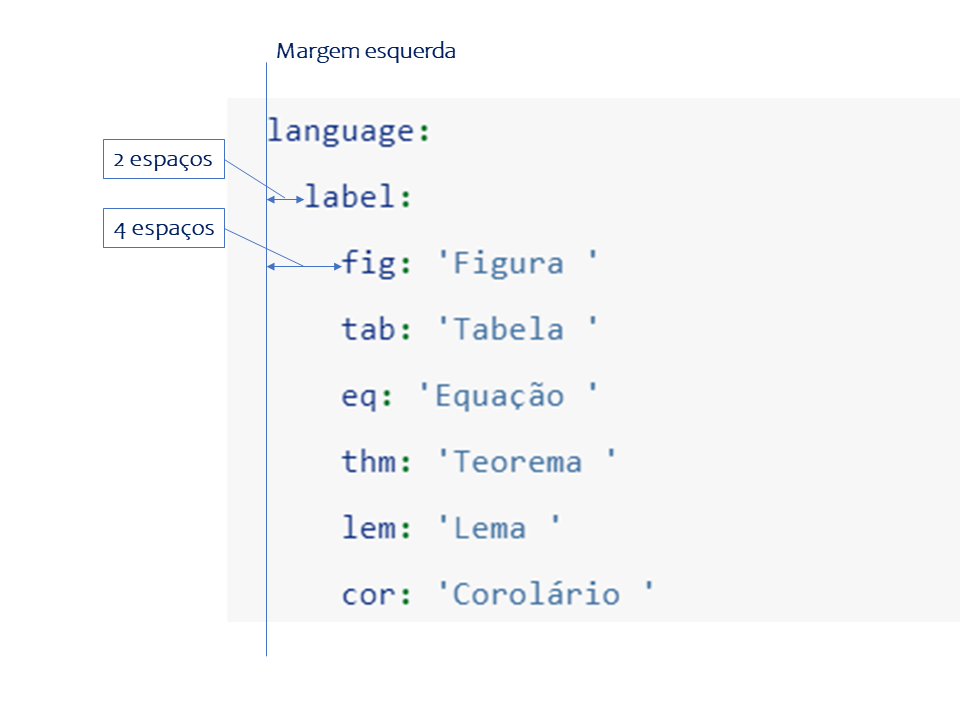
\includegraphics[width=400pt]{image/indent-bookdown} \caption{Exemplo de indentação no arquivo \texttt{\_bookdown.yml}.}\label{fig:ident-bookdown}
\end{figure}

\hypertarget{output}{%
\chapter{\texorpdfstring{O arquivo \texttt{\_output.yml}}{O arquivo \_output.yml}}\label{output}}

Este é um exemplo do conteúdo do arquivo \texttt{\_output.yml}

\begin{Shaded}
\begin{Highlighting}[]
\AttributeTok{bookdown:}\FunctionTok{:gitbook}\KeywordTok{:}\CommentTok{ \#https://bookdown.org/yihui/bookdown/html.html\#gitbook{-}style}
\AttributeTok{  }\FunctionTok{css}\KeywordTok{:}\AttributeTok{ style.css}\CommentTok{ \#arquivo .css}
\AttributeTok{  }\FunctionTok{split\_by}\KeywordTok{:}\AttributeTok{ chapter}\CommentTok{ \#rmd, none, chapter, section, chapter+number, section+number}
\AttributeTok{  }\FunctionTok{split\_bib}\KeywordTok{:}\AttributeTok{ }\CharTok{yes}\CommentTok{ \#yes: adiciona as referências em cada página}
\AttributeTok{  }\FunctionTok{includes}\KeywordTok{:}
\AttributeTok{    }\FunctionTok{in\_header}\KeywordTok{:}\AttributeTok{ ga.html}\CommentTok{ \#incluir códigos no HEAD do html, por exemplo, google analytics}
\AttributeTok{  }\FunctionTok{config}\KeywordTok{:}
\AttributeTok{    }\FunctionTok{toc}\KeywordTok{:}
\AttributeTok{      }\FunctionTok{collapse}\KeywordTok{:}\AttributeTok{ none}\CommentTok{ \#subsection, section, none}
\AttributeTok{      }\FunctionTok{scroll\_highlight}\KeywordTok{:}\AttributeTok{ }\CharTok{yes}
\FunctionTok{      before}\KeywordTok{: }\CharTok{|}
\NormalTok{        \textless{}li\textgreater{}\textless{}a href="./"\textgreater{}Exemplo mínimo de um e{-}book\textless{}/a\textgreater{}\textless{}/li\textgreater{}}
\FunctionTok{      after}\KeywordTok{: }\CharTok{|}
\NormalTok{        \textless{}li\textgreater{}\textless{}a href="https://github.com/rstudio/bookdown" target="blank"\textgreater{}Publicado com bookdown\textless{}/a\textgreater{}\textless{}/li\textgreater{}}
\AttributeTok{    }\FunctionTok{toolbar}\KeywordTok{:}
\AttributeTok{      }\FunctionTok{position}\KeywordTok{:}\AttributeTok{ fixed}\CommentTok{ \#fixed, static}
\AttributeTok{    }\FunctionTok{search}\KeywordTok{:}\AttributeTok{ }\CharTok{yes}
\AttributeTok{    }\FunctionTok{fontsettings}\KeywordTok{:}
\AttributeTok{      }\FunctionTok{theme}\KeywordTok{:}\AttributeTok{ white}\CommentTok{ \#white, night, sepia}
\AttributeTok{      }\FunctionTok{family}\KeywordTok{:}\AttributeTok{ sans}\CommentTok{ \#sans, serif}
\AttributeTok{      }\FunctionTok{size}\KeywordTok{:}\AttributeTok{ }\DecValTok{2}\CommentTok{ \#1 a 4}
\AttributeTok{    }\FunctionTok{download}\KeywordTok{:}\AttributeTok{ }\CharTok{null}
\AttributeTok{    }\FunctionTok{sharing}\KeywordTok{:}
\AttributeTok{      }\FunctionTok{whatsapp}\KeywordTok{:}\AttributeTok{ }\CharTok{yes}
\AttributeTok{      }\FunctionTok{facebook}\KeywordTok{:}\AttributeTok{ }\CharTok{yes}
\AttributeTok{      }\FunctionTok{twitter}\KeywordTok{:}\AttributeTok{ }\CharTok{yes}
\AttributeTok{      }\FunctionTok{linkedin}\KeywordTok{:}\AttributeTok{ }\CharTok{no}
\AttributeTok{      }\FunctionTok{weibo}\KeywordTok{:}\AttributeTok{ }\CharTok{no}
\AttributeTok{      }\FunctionTok{instapaper}\KeywordTok{:}\AttributeTok{ }\CharTok{no}
\AttributeTok{      }\FunctionTok{vk}\KeywordTok{:}\AttributeTok{ }\CharTok{no}
\AttributeTok{      }\FunctionTok{all}\KeywordTok{:}\AttributeTok{ }\KeywordTok{[}\StringTok{\textquotesingle{}whatsapp\textquotesingle{}}\KeywordTok{,}\AttributeTok{ }\StringTok{\textquotesingle{}facebook\textquotesingle{}}\KeywordTok{,}\AttributeTok{ }\StringTok{\textquotesingle{}twitter\textquotesingle{}}\KeywordTok{,}\AttributeTok{ }\StringTok{\textquotesingle{}linkedin\textquotesingle{}}\KeywordTok{]}
\AttributeTok{    }\FunctionTok{info}\KeywordTok{:}\AttributeTok{ }\CharTok{yes}
\end{Highlighting}
\end{Shaded}

Para a saída GitBook (\texttt{bookdown::gitbook}), algumas das configurações são as seguintes:

\begin{itemize}
\tightlist
\item
  \texttt{css}: para fornecer um ou mais arquivos CSS personalizados.
\item
  \texttt{split\_by}: especifica como dividir os arquivos HTML em múltiplas páginas. As opções são:

  \begin{itemize}
  \tightlist
  \item
    \texttt{rmd}: cada arquivo Rmd cria um arquivo HTML.
  \item
    \texttt{none}: não separa o arquivo, ou seja, o livro todo está contido em um único HTML.
  \item
    \texttt{chapter}: separa para cada cabeçalho de primeiro nível.
  \item
    \texttt{section}: separa para cada cabeçalho de segundo nível.
  \item
    \texttt{chapter+number} and \texttt{section+number}: similar a \texttt{chapter} e \texttt{section}, ma os arquivos são numerados.
  \end{itemize}
\item
  \texttt{split\_bib}: se \texttt{split\_bib\ =\ yes} adiciona as referências ao final de cada página. Caso \texttt{split\_bib\ =\ no}, as referências são colocadas apenas em uma página separada.
\item
  \texttt{includes}: possibilita incluir um código HTML no arquivo de saída. Uma opção comum é incluir o código do Google Analytics (veja mais em \href{http://tolentino.pro.br/post/google-analytics/}{Google Analytics no Bookdown})
\end{itemize}

As opções indentadas dentro de \texttt{config} são:

\begin{itemize}
\tightlist
\item
  \texttt{toc}: controla o sumário (table of contents), que aparece no lado direiro da tela.

  \begin{itemize}
  \tightlist
  \item
    \texttt{collapse}: os valores possíveis são: \texttt{subsection}, que desdobra o sumário até o terceiro nível, \texttt{section} que desdobra o sumário até o segundo nível e \texttt{none}, que desdobra até o primeiro nível.
  \item
    \texttt{scroll\_highlight}: se \texttt{yes}, destaca o item atual do sumário enquanto você rola a página.
  \item
    \texttt{before} and \texttt{after}: adiciona itens antes e/ou depois do sumário.
  \end{itemize}
\item
  \texttt{toolbar}: controla o comportamento da barra superior.

  \begin{itemize}
  \tightlist
  \item
    \texttt{position}: os valores podem ser \texttt{fixed}, que fixa a barra superior e ela estará sempre visível mesmo quando a página é rolada, ou \texttt{static}, que não rola a barra junto com a página, ou seja, ela não estará mais visível conforme a página é rolada.
  \end{itemize}
\item
  \texttt{search}: se \texttt{yes}, adicoina um botão de busca na barra superior.
\item
  \texttt{fontsettings}: ajusta os valores iniciais para o tema e fonte. Para desativar, ajuste o valor para \texttt{null}.

  \begin{itemize}
  \tightlist
  \item
    \texttt{theme}: os valores são \texttt{white} para um tema claro, \texttt{night} para um tema escuro e \texttt{sepia} para um tema com efeito envelhecido.
  \item
    \texttt{family}: \texttt{serif} para uma fonte serifada \href{https://pt.wikipedia.org/wiki/Serifa}{(O que é uma fonte serifada?)} ou \texttt{sans} para uma fonte não serifada.
  \item
    \texttt{size}: tamnho da fonte, entre 1 e 4
  \end{itemize}
\item
  \texttt{download}: permite o download do e-book em outros formatos, como PDF ou EPUB. Os valores devem ser colcoados em um vetor, por exemplo, \texttt{{[}"pdf",\ "epub"{]}}. Caso download seja definido como \texttt{null}, o programa irá procurar pelos arquivos no diretório de saída e adicionar automaticamente. Para desabilitar o download, definir como \texttt{no}.
\item
  \texttt{sharing}: Adiciona botões para compartilhamento em redes sociais. Para desativar, definir como \texttt{no}.

  \begin{itemize}
  \tightlist
  \item
    \texttt{whatsapp}: se definido como \texttt{yes}, um botão para compartilhar a página no whatsapp irá aparecer na barra superior. Outras opções de redes sociais são: facebook, twitter, linkedin, weibo, instapaper e vk.
  \item
    \texttt{all}: ícones das redes sociais que irão aparacer no menu \emph{dropdown} de compartilhamento.
  \end{itemize}
\item
  \texttt{info}: botão de informação que lista os atalhos do teclado. Para desativar, definir como \texttt{no}.
\end{itemize}

\hypertarget{index0}{%
\chapter{\texorpdfstring{O arquivo \texttt{index.Rmd}}{O arquivo index.Rmd}}\label{index0}}

Este é o cabeçalho YAML do arquivo \texttt{index.Rmd}

\begin{Shaded}
\begin{Highlighting}[]
\PreprocessorTok{{-}{-}{-} }
\FunctionTok{title}\KeywordTok{:}\AttributeTok{ }\StringTok{"Publicando e{-}book com o bookdown"}
\FunctionTok{author}\KeywordTok{:}\AttributeTok{ }\StringTok{"João B. Tolentino Jr."}
\FunctionTok{date}\KeywordTok{:}\AttributeTok{ }\StringTok{"2022{-}03{-}04"}
\FunctionTok{description}\KeywordTok{:}\AttributeTok{ }\StringTok{"Este é um exemplo de um livro publicado com o pacote **bookdown** no formato *gitbook*"}
\FunctionTok{cover{-}image}\KeywordTok{:}\AttributeTok{ image/cover.jpg}
\FunctionTok{apple{-}touch{-}icon}\KeywordTok{:}\AttributeTok{ image/cover.jpg}
\FunctionTok{favicon}\KeywordTok{:}\AttributeTok{ image/favicon.ico}
\FunctionTok{url}\KeywordTok{:}\AttributeTok{ }\StringTok{\textquotesingle{}https\textbackslash{}://curso{-}bookdown.tolentino.pro.br\textquotesingle{}}
\FunctionTok{site}\KeywordTok{:}\AttributeTok{ bookdown::bookdown\_site}
\FunctionTok{documentclass}\KeywordTok{:}\AttributeTok{ book}
\FunctionTok{bibliography}\KeywordTok{:}\AttributeTok{ }\KeywordTok{[}\AttributeTok{book.bib}\KeywordTok{,}\AttributeTok{ packages.bib}\KeywordTok{]}
\FunctionTok{biblio{-}style}\KeywordTok{:}\AttributeTok{ apalike}
\FunctionTok{link{-}citations}\KeywordTok{:}\AttributeTok{ }\CharTok{yes}
\PreprocessorTok{{-}{-}{-}}
\end{Highlighting}
\end{Shaded}

\begin{itemize}
\tightlist
\item
  \texttt{title}: título do e-book.
\item
  \texttt{author}: nome do(s) autor(es) do e-book
\item
  \texttt{date}: data de publicação. Para buscar automaticamente data em qe=ue foi feita a última modificação, use a função \texttt{Sys.Date()}
\item
  \texttt{description}: um descrição sucinta utilizada pelos buscadores (SEO)
\item
  \texttt{cover-image}: uma imagem de capa para o e-book que irá aparecer quando compartilhar o link nas redes sociais.
\item
  \texttt{apple-touch-icon}: para IOS, o ícone quando o website é adiconada na tela inicial
\item
  \texttt{favicon}: ícone mostrado na barra de endereços ou nas abas do navegador.
\item
  \texttt{url}: a \emph{url} do website do e-book. Atenção para a barra esquerda que deve ser adicionada antes de dois pontos do endereço.
\item
  \texttt{site}: para renderizar o e-book no RStudio, definir a opção como \texttt{bookdown::bookdown\_site}.
\item
  \texttt{documentclass}: definir como \texttt{book}.
\item
  \texttt{bibliography}: arquivos que contém a bibliografia, no formato *.bib
\item
  \texttt{biblio-style}: estilo das citações.
\item
  \texttt{link-citation}: definir como \texttt{yes} para as citações também serem links.
\end{itemize}

\hypertarget{latex}{%
\chapter{Latex}\label{latex}}

\end{document}
